%!TEX root = ../../master.tex

\section{Service Discovery}
When microservices are deployed to a cloud computing infrastructure, the problem of knowing where each particular service is located arises, e.g. their network location being an IP and port. This problem arises because of the dynamic infrastructure where services can be scaled, fail and new ones scheduled on different nodes, which leads to different network locations. Because of this dynamic architecture, a solution to locate and discover services is needed. 

\subsection*{Client-Side Service Discovery}
Client-side service discovery refers to clients being responsible for determining the network locations of available services and load balance requests across them. To do this, the client queries a service registry, which has an internal database with the available services. The client uses a load-balancing algorithm to select the appropriate available service and makes a request. This pattern is shown in Figure~\ref{fig:client_side_service_discovery}.

\begin{figure}[H]
    \centering
    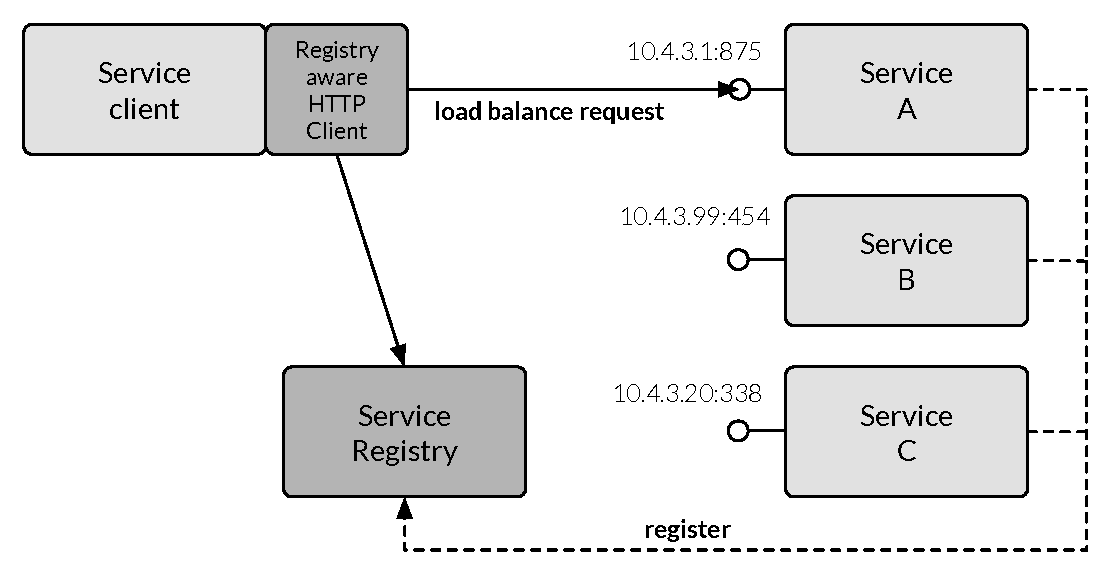
\includegraphics[width=9cm]{figures/client_side_service_discovery}
    \caption{Client Side Service Discovery \cite{servicediscovery}}
    \label{fig:client_side_service_discovery}
\end{figure}

\noindent 
Before the service registry can be used to full effect, each service in the architecture needs to be registered. When a service starts up, it is announced on the network, and the service registry adds the service to the database. If the service for some reason gets terminated, the service registry needs to be notified. The service registry maintains the database by using a heartbeat mechanism to check if services still are available and ready to respond to requests. An example of the client-side service discovery is Netflix's open source tool, Eureka. Eureka provides an HTTP REST interface and together with another Netflix tool, the client side load balancer called Ribbon, the service registration and load balancing is handled.

\subsection*{Server-Side Service Discovery}
In server-side service discovery, it is no longer the client's responsibility to query the service registry. Instead, it is the load balancer that queries the service registry and routes each request to an available service. Registration and deregistration are handled in the same way as the client-side service discovery. 

\begin{figure}[H]
    \centering
    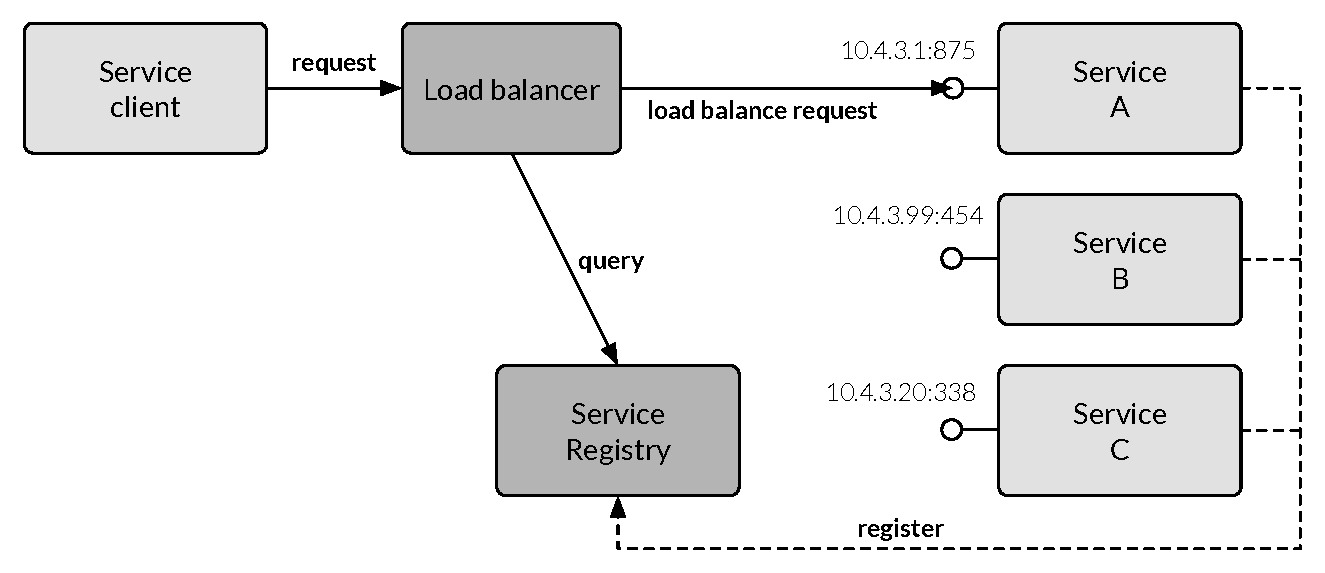
\includegraphics[width=11cm]{figures/server_side_service_discovery}
    \caption{Server Side Service Discovery \cite{servicediscovery}}
    \label{fig:server_side_service_discovery}
\end{figure}

\noindent An example of applied server-side service discovery is Kubernetes. Kubernetes runs a proxy on each host in the cluster. Richardson describes the role of the proxy: \textit{"The proxy plays the role of a server-side discovery load-balancer"} \cite[p. 7]{servicediscovery}. Nommensen describes the server-side service discovery flow of Kubernetes: \textit{"in order to make a request to a service, a client routes the request via the proxy using the host's IP address and the service's assigned port"} \cite{servicediscovery_nommensen}. This results in the request transparently being forwarded by the proxy to an available service running somewhere in the cluster. \\